\documentclass[twocolumn]{article}

\def\topfraction{.85}
\def\dbltopfraction{.85}
\def\textfraction{.12}

\usepackage{natbib}
\usepackage{amsmath}
\usepackage[utf8]{inputenc}
\usepackage{graphicx}
\usepackage{url}
\usepackage{rotating}

\def\npup{\ensuremath{S}}
\def\nmaj{\ensuremath{D}}
\def\nprof{\ensuremath{A}}
\def\ngrad{\ensuremath{A^\text{pg}}}
\def\ngrant{\ensuremath{G}}
\def\nisi{\ensuremath{P^\text{WoS}}}
\def\nscielo{\ensuremath{P^\text{S}}}

\def\der#1#2{\frac{\mathrm{d}\,{#1}}{\mathrm{d}#2}}
\def\pder#1#2{\frac{\partial\,{#1}}{\partial#2}}

\def\Fnew{\ensuremath{F^\text{new}}}
\def\nal{\ensuremath{N_\text{pub}}}
\def\nal{\ensuremath{N_\text{alumnos}}}
\def\nal{\ensuremath{N_\text{alumnos}}}
\def\eqref#1{Eq.~(\ref{eq:#1})}
\makeatletter
\def\eqsref#1#2{Eqs.~(\ref{eq:#1}--\ref{eq:#2})}
\makeatother

\usepackage{geometry}
\geometry{left=16mm,top=16mm,right=20mm,bottom=20mm}

\title{Direct Government Contribution to Chilean universities}
\author{Régis Lachaume}

\begin{document}

\maketitle

\section{Introduction}
Aporte Fiscal Directo, or Direct Government Contribution, hereafter AFD.

\section{Mathematical analysis}
The funding consists of two parts: 5\% is allotted to Universities according to a measurement of their current efficiency and 95\% according to their past share of the funding.

\subsection{Efficiency-dependent funding (5\%)}
\subsubsection{Calculation}
\label{sec:metrics}

Art. 2 of Decree with Force of Law 4 of 1980, with modifications from Art. 1 of Ministry of Education Decree 116 of 2002, indicates that 5\% part of the total funding of year $n + 1$ is distributed to University $i$ according to its metrics reported after year $n$\footnote{Some are from year $n$ and others from year $n-1$.}. They involve 
\begin{itemize}
\item $\npup_{i,n}$, the number of undergraduate students (``estudiantes de pregrado'');
\item $\nmaj_{i,n}$, the number of bachelor degree disciplines (``carreras'');
\item $\nprof_{i,n}$, the number of equivalent full-time academic staff (``académicos''), i.e. professors;
\item $\ngrad_{i,n}$, the number of equivalent full-time academic staff with a post-graduate title such as master or a PhD; 
\item $\ngrant_{i,n}$, the number of research grants (``proyectos'');
\item $\nisi_{i,n}$, the number of Web of Science publications (WoS)\footnote{At the time of the Decree 116 it was known as ISI}; 
\item and $\nscielo_{i,n}$, the number of non-WoS publications indexed by the Scientific Electronic Library Online (Scielo) Chile. 
\end{itemize}

The metrics, defined in the aformentioned decrees, are ratios meant to measure an output v. staff efficiency\footnote{While the number of publications is defined by the number of WoS plublications plus one third of Scielo one by Ministry of Education Decree 116 of 2002, the Ministry has consistently used factor 0.33 instead of 1/3 for the calculation.}
\begin{subequations}
\begin{align}
    x_{i,n,1} &= \npup_{i,n} / \nmaj_{i,n},  \label{eq:x1}             \\
    x_{i,n,2} &= \npup_{i,n} / \nprof_{i,n},                           \\ 
    x_{i,n,3} &= \ngrad_{i,n} / \nprof_{i,n},                          \\
    x_{i,n,4} &= \ngrant_{i,n} / \nprof_{i,n},                         \\
    x_{i,n,5} &= (\nisi_{i,n} + \frac{33}{100} \nscielo_{i,n}) / \nprof_{i,n}
\end{align}
\end{subequations}

According to Art. 3 of Ministry of Education Decree 128 of 1991,  the
evaluation formula renormalises the aforemention ratios in this
way\footnote{Although not specified by the decree, the Ministry has
consistently used the population variance, not the sample variance, for the calculation.}:
\begin{subequations}
\begin{align}
    \mu_{n,k}    &= \frac1N\sum_j x_{j,n,k}\qquad\text{(mean)} \label{eq:mu}\\
    \sigma_{n,k} &= \sqrt{\frac 1N \Big(\sum_j x_{j,n,k}^2\Big) - N\mu_{n,k}^2}\qquad\text{(std. dev.)} \label{eq:sigma}\\
    \xi_{i,n,k}  &= \frac{x_{i,n,k} - \mu_{n,k} }{\sigma_{n,k}} 
\qquad\text{(reduced coeff.)} \label{eq:xi}\\
    y_{i,n,k}    &= \exp \left[ -\frac 75 + \frac{\xi_{i,n,k}}4  \right]^3 \label{eq:transform}
\end{align}
\end{subequations}
where $N$ is the total number of universities.
The transform in \eqref{xi} ensures that Universities are compared by how many standard deviations they are from the mean. The exponential in \eqref{transform} is supposed to simulate a biological growth. Figure~\ref{fig:transform} displays the exponential nature of the rating.

Art.~2 of Decree with Force of Law~4 of 1980 indicates that 5\% of the funding
is indexed on a weighted average of the metrics $y_{i,n,k}$ (k in $1\cdots5$)
(see Sect.~\ref{sec:metrics}). The weights $c_k$ may vary from year to year,
but have been constant since 1998 with $c = (0.01, 0.14, 0.24, 0.25, 0.35)$.  University $i$ is thus assigned a score
\begin{subequations}
\begin{align}
    y_{i,n}    &= \sum_k c_k y_{i,n,k}. \label{eq:y}\\
\intertext{and, using the total score}
    y_{n}      &= \sum_i y_{i,n},\\
\intertext{a funding share}
    f_{i,n}    &= \frac{y_{i,n}}{y_{n}} \label{eq:f}
\end{align}
\end{subequations}


\begin{figure}[t]
\centering
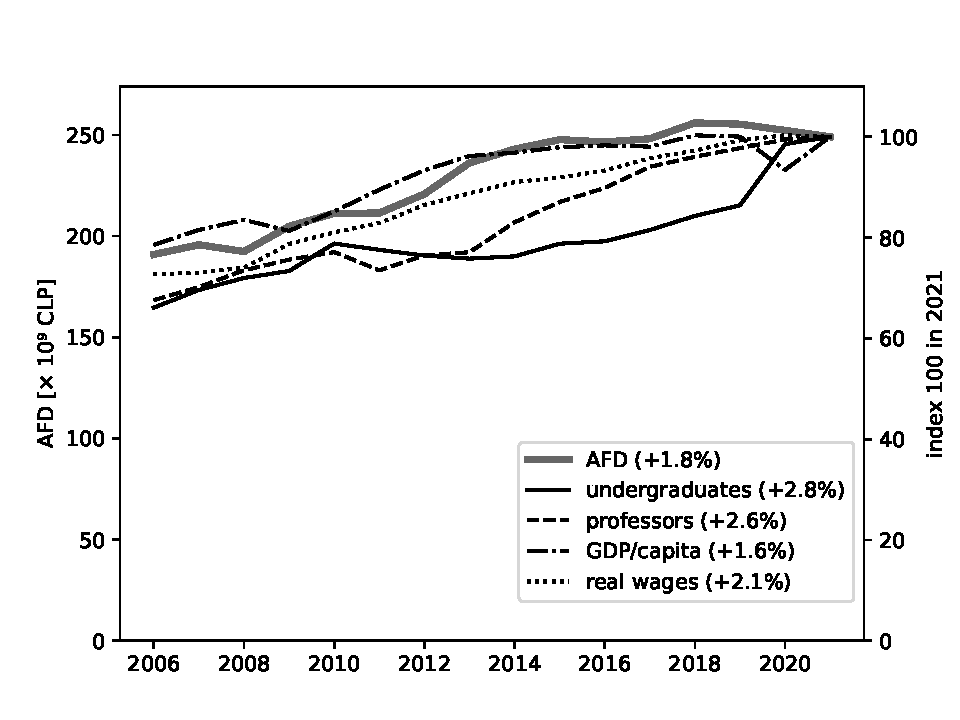
\includegraphics[width=\linewidth]{pdf/total-afd-timeseries.pdf}
\caption{Evolution of total direct State funding to traditional Chilean Universities, in 2020 pesos (inflation-corrected) compared to the evolution of the GDP per capita (World Bank data), the mean real wage (Instituto Nacional de Estadísticas data), the number of undergraduate students and the number of professors.}
\label{fig:total-afd}
\end{figure}

\begin{figure*}[p]
\centering
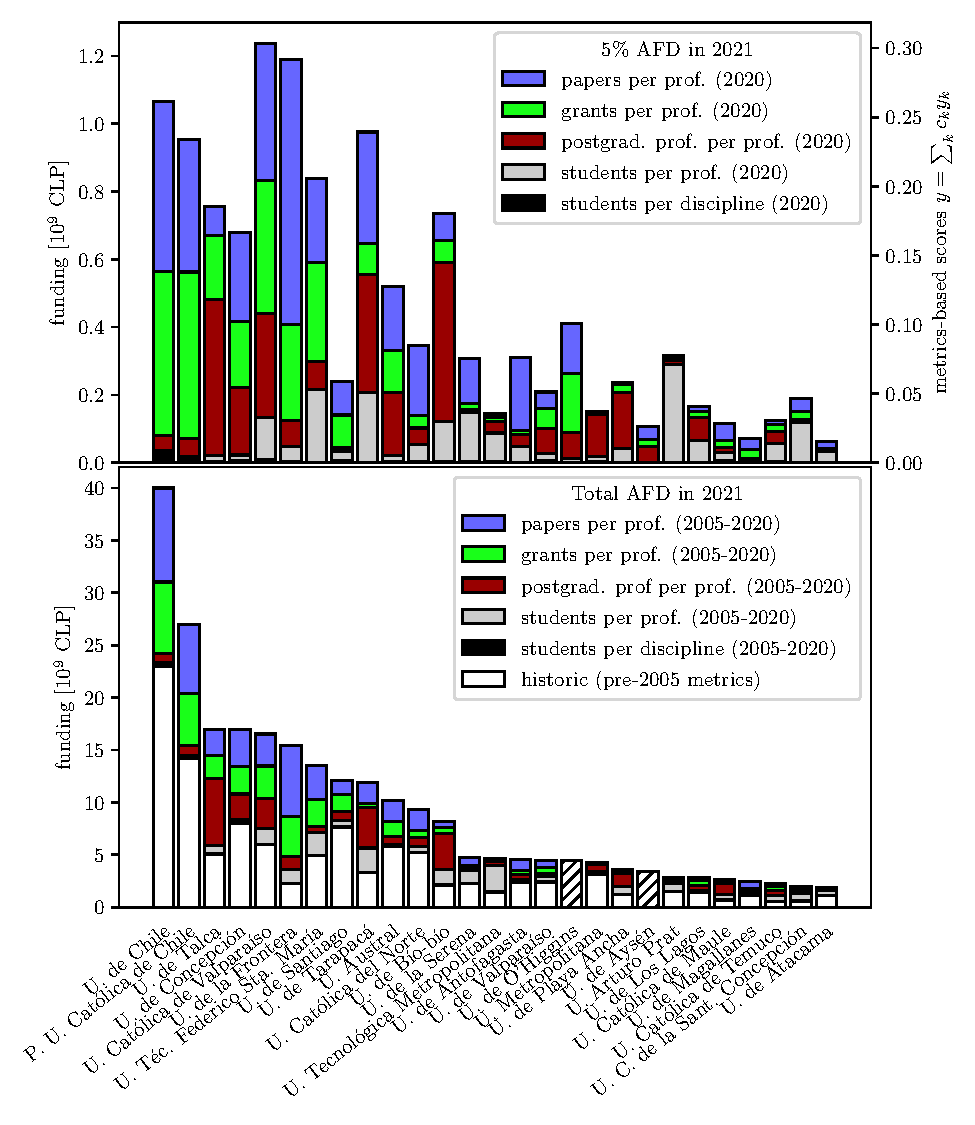
\includegraphics{pdf/afd-coefficients.pdf}
\caption{Contribution of each metric to the AFD funding of traditional Chilean universities in 2021. \textit{Top panel:} contributions of 2020 metrics to the 5\%. \textit{Bottom panel:} contributions of the recent metrics and historic pre-2005 ones to the total funding. \textit{Left axis:} thousand million Chilean pesos, of the order of million US dollars. \textit{Right axis:} university scores $c_k y_k$ and its total $y = \sum c_k y_k$. The historic funding is not shown for newly minted universities of O'Higgins and Aysén.  The data used to produce the top panel of this figure can be found in Table~\ref{tab:calcdetail}.}
\label{fig:coeff}
\end{figure*}

The 2021 funding via the 5\% is shown in the top panel of Figure~\ref{fig:coeff}, with the contributions of each metrics.

\subsubsection{Marginal earnings}
\label{sec:marginal} 

\begin{figure*}[p]
\centering
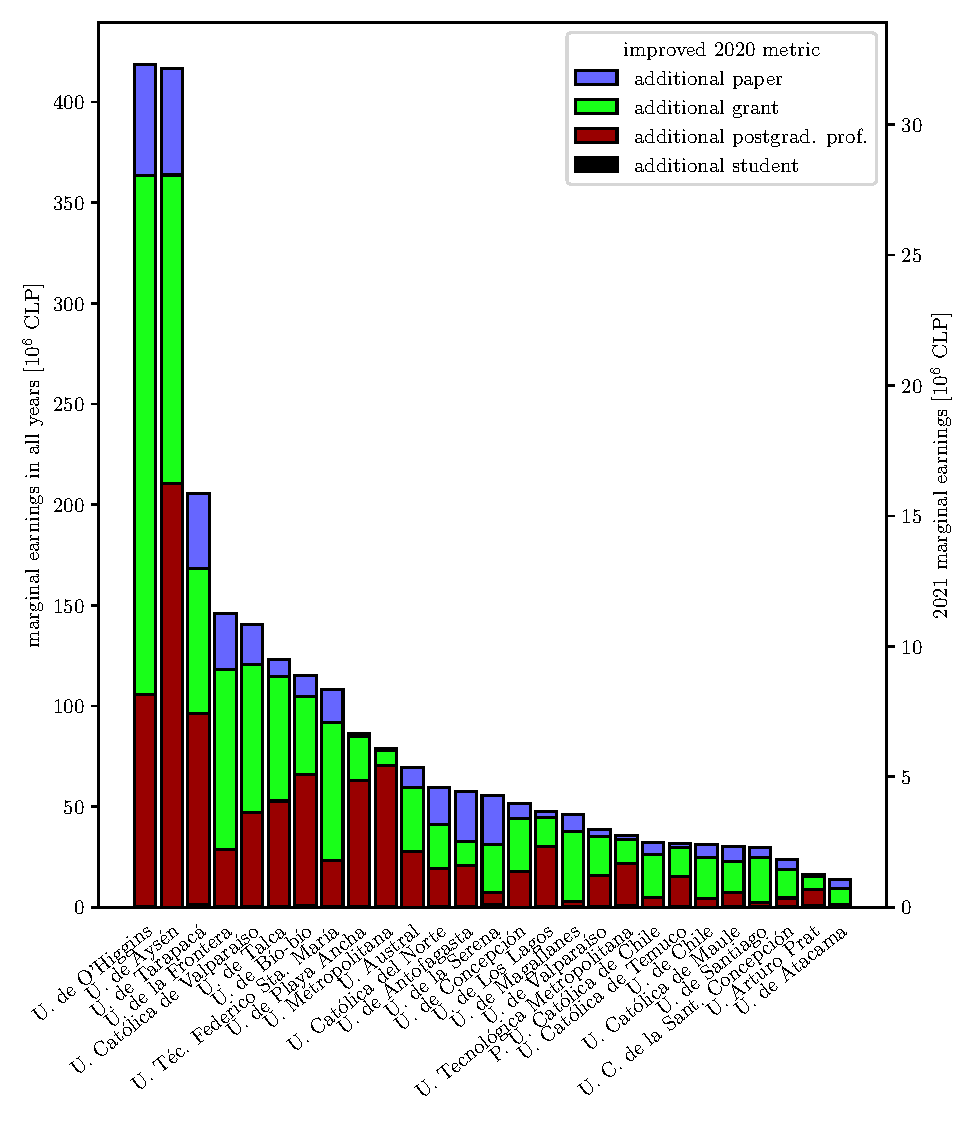
\includegraphics{pdf/marginal-earnings.pdf}
\caption{Marginal earnings of traditional Universities for each of the following improvements reported in 2020: one additional undergraduate student, one additional one-year contract of a postgraduate professor instead of one without a postgraduate title, one additional one-year research grant, one additional WoS (ex-ISI) publications.  \textit{Left axis:} present value of total earnings in million Chilean pesos, assuming a yearly depreciation of 5\% in real terms and 2\% increase of total funding by the State. \textit{Right axis:} earnings in year 2021. The data used to produce this figure can be found in Table~\ref{tab:marginal}.}
\label{fig:marginal}
\end{figure*}

In this section, I focus on a yearly snapshot and drop the $n$ index in the formulae.  I examine the case where university $i$ decides to increase one of its ratios number $k$ by a small number of standard deviations $\Delta\xi_{i,k}$, so that the ratio $x_{i,k}$ improves by $\Delta x_{i,k} = \sigma_k\Delta\xi_{i,k}$.

For any university $j$, the new value of the score $y_{j,k}$ is usually modified because the mean and standard deviation are changed via $x_{i,k}$.  The difference $\Delta y_{j,k}$ is given by differentiating \eqref{transform}, and in turn \eqsref{mu}{xi} on which it depends.
The calculation, detailed in  in Appendix~\ref{sec:calculus}, yields
\begin{equation}
    \frac{\Delta y_{j,k}}{y_{j,k}} = 
        \frac34 \left(\frac{\xi_{j,k}}4 -  \frac75\right)^2 
        \left(
            \delta_{ij} 
          - \frac 1N - \frac{\xi_{i,k}\xi_{j,k}}{N}
        \right)
        \Delta \xi_{i,k},
        \label{eq:modif}
\end{equation}
where $\delta_{ij} = 1$ if universities $i$ and $j$ are the same and zero otherwise.

The meaning of \eqref{modif} is the following:
\begin{enumerate}
    \item \emph{$(\xi_{j,k}/4 - 7/5)^2$ factor}:  The relative improvement depends on the relative standing of the University in the ranking.  A university lagging behind by 2 standards deviations gets a relative improvement 4,5 times higher than a university standing out by 2 standard deviations. However, due to the exponential nature of $y$ dependency on $\xi$, the absolute improvement is close to zero for universities with a low standing ($\xi \ll 0$) and large for the top tier ones ($\xi \gg 0$).
    \item \emph{$\delta_{ij}$ term:} University $i$ generally benefits from an increase of its own ratio $\Delta x_{i,k}$: the $\delta_{ij}$ (= 1 for $i = j$) term in the equation is the only one that is not in $1/N$ and thus dominates. However, if $|\xi_{i,k}| > \sqrt{N - 1} \approx 5$ standard deviations, University would lose from improving.  Nevertheless, the data of the Ministery from 2006 to 2020 can be used to show that the highest deviation any of the ratio has ever reached is 3.7.
    \item University $j$ may benefit from, or be harmed by, the improvement of University $i$.  There are two effects at play.  
    \begin{enumerate}
    \item \emph{$1/N$ term}: The increase of the mean, would on its own hurt all other universities as their position relative to the mean $\xi_{j,k}$ would drop (see the $1/N$ term in the equation).  
    \item \emph{$\xi_{i,j}\xi_{j,k}/N$ term}: However, the modification of the standard deviation works both ways. Intuitively, if a university with a high $\xi_{i,k} > 0$ ($x_{i,k} > \mu_k$) improves, it will increase the standard deviation, so that all universities deviate less from the mean: other universities with $\xi_{j,k} > 0$ will lose some of their good standing and lower tier ones with $\xi_{j,k} < 0$ will decrease their lag . Conversely, on can see that the improvement of a University with a lower rank $\xi_{j,k} < 0$, by decreasing the standard deviation of the sample when it goes closer to the mean, will help those with good standing to stand out more and harm other lower tier ones. 
\end{enumerate}
    For both effects combined, University $j$ benefits if $\xi_{i,k}\xi_{j,k} < -1$ and is harmed otherwise. 
\end{enumerate}

To determine the additional funding fraction $\Delta f_j$, let's propagate 
\eqref{modif} into \eqsref{y}{f}:
\begin{equation}
    \frac{\Delta f_j}{f_j} = c_k \left[
                     \left(1 - \frac{y_{j}}y\right)\frac{\Delta y_{j,k}}{y_{j}}
                    - \sum_{l \ne j} \frac{y_l}y \frac{\Delta y_{l,k}}{y_l}
                 \right].
    \label{eq:deltafi}
\end{equation}
The first term in the square brackets has the same sign as $\Delta y_{j,k}$ because, by definition, $y_j < y$.  In most cases, the second term is smaller than the first one because the $\Delta y_{l,k}$ partially cancel out (some positives and some negatives) and $y_l < y$. It means that the funding received by a university that has an improved rating normally receives additional funding.  It is possible, though, that a university with a very small $\Delta y_{j,k}$ (e.g. $\xi_{j,k} < -2$) will be harmed by increasing its score, because the other, larger, $\Delta y_{l,k}$ coould lead to a second term larger than the first term under these circumstances. In years 2006--2021, it has happened exactly twice for Universidad de Aysén, who would have lost 14,000 and 1,000 pesos in 2020 and 2021, respectively, had it had one undergraduate student more in 2018 and 2019. It happens that the university had the two worst standard deviations observed for any metrics with $\xi_{\text{U. de Aysén},2} \approx -2.8$.

The previous determination is an approximation, valid for small values of $\Delta \xi$. To obtain the exact value, the calculations in \eqsref{x1}{afd} are done with the metrics provided by the Ministry (see Sect.~\ref{sec:metrics}) and for the same ones with additional students, professors with a postgraduate title, publications, or grants.  The difference is the marginal earning. This exact calculation is reported in Fig.~\ref{fig:marginal} (scale on the right axis).

\subsection{Historic (95\%) and total funding}

\subsubsection{Evolution of total funding}

The total funding in year $n$, $F_{n}$, is a slowly increasing series (see Fig.~\ref{fig:total-afd}). In half of the years it approximately follows the consumer price index, but it has received a modest boost in other years.  The average inflation-corrected increase has been $1.8$\% per year in period 2006--2021. This increases matches the increase in undergraduate students ($+2.8\%$ in 2004--2019), professors ($+2.6\%$ in 2005--2020), real wages ($+2.1\%$ in 2006--2021), and GDP per capita ($+1.6$\% in 2006--2021). Table~\ref{tab:macro} in Appendix~\ref{sec:macro} gives an overview of the main macroeconomic quantities in this period. Note that the pre-pandemic trends for macroeconomic data and AFD evolution were about 0.2\% higher. 
 
Increase in standard of living and student population are long-term trends that I would expect to hold for at least the next decade, so I assume that University funding by the State will still follow this trend. For predictions, beyond 2021, I will therefore take
\begin{equation}
    F_{n+1} = (1+q) F_n, \label{eq:F}
\end{equation}
where $q = 2$\%.

\subsubsection{University funding (5\% and 95\%)}

Let $F_{i,n}$ be the funding received by university $i$ at year $n$. Art. 2 of
Decree with Force of Law 4 of 1980 indicates that 5\% of the funding is indexed
on metrics $y_{i,n,k}$ and 95\% of the funding is related to the previous year's
share of the total funding.  So,

\begin{align}
    F_{i,n+1} &= \frac{19F_{i,n}}{20F_{n}}\left(F_{n+1} - \Fnew_{n+1}\right)
               + \frac{y_{i,n}}{20y_n} F_{n+1}.
        \label{eq:afd}
\end{align}
where $F_{n+1}^\text{new}$ is the part of the 95\% apportionned to newly admitted traditional universities.  In the period 2006--2021, it has been nonzero in 2018 when State Universities of O'Higgins and Aysén where included (Decree 228 of 2017).  

\subsubsection{Funding by metric}  

\begin{figure*}[p]
\centering
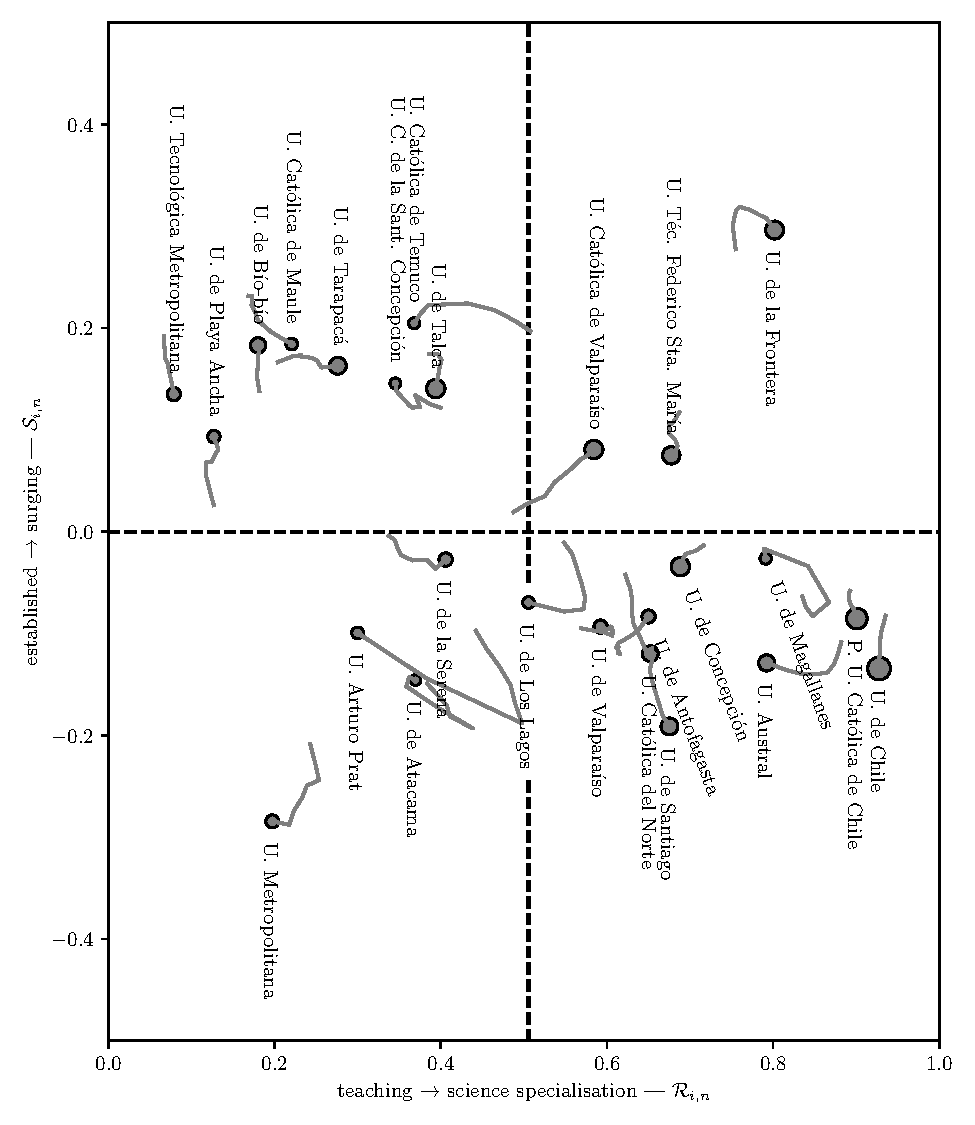
\includegraphics{pdf/afd-specialisation.pdf}
\caption{Classification of traditional universities according to their teaching v. science specialisation and their established v. surging status. The two newly created institutions have not been included. \textit{Circles:} 2021 standing, area is proportional to the total AFD funding received in 2021. \textit{Gray tracks:} evolution of the universities through years 2014--2021. \textit{Horizontal axis:} research index, i.e. ratio of funding originating from the 2005--2020 science metrics (number of grants and papers) to the one from all 2005--2020 metrics. The vertical line indicates the median value. \textit{Vertical axis:} surging index, i.e. ratio of funding obtained from recent metrics to total funding minus its expected steady state value.  }
\label{fig:classification}
\end{figure*}

Funding received in virtue of a given metric in a given year still yields additional funding in the subsequent years since it propagates via the 95\%.

For an analysis of the strengths and weaknesses of each Universities, it is useful to determine what part of the total AFD funding originates from ``historic'' funding at year $n_0$ and which parts originate from each of the metrics computed for the funding of years $n_0 + 1$ to $n$. Let $H_{i,n}$ be the share of ``historic'' funding of university $i$ in year $n$ and $F_{i,n,k}$ that of the metric number $k$. They can be determined via the initial conditions and recurrence relations:
\begin{subequations}
\begin{align}
  H_{i, n_0}  &= F_{i, n_0},\\
  H_{i,n+1}   &= \frac{19H_{i,n}}{20F_n}   \left(F_{n+1}-\Fnew_{n+1}\right),
                    \label{eq:recH}\\
  F_{i,n_0,k} &= 0,\\
  F_{i,n+1,k} &= \frac{19F_{i,n,k}}{20F_n} \left(F_{n+1} - \Fnew_{n+1}\right)
                  + \frac{c_k y_{i,n,k}}{20y_n} F_{n+1}
                    \label{eq:recF}\\
              &\qquad\qquad \text{for $1 \le k \le 5$}. \notag
\end{align}
\end{subequations}
It is straighforward to check that $F_{i,n} = H_{i,n} + \sum_k F_{i,n,k}$ since the six recurrence equations (Eqs.~\ref{eq:recH}~\& \ref{eq:recF}) sum to Eq.~(\ref{eq:afd}).  The contribution of the pre-2006 funding and the 2005--2020 values of each metric to the total funding is given in the bottom panel of Fig.~\ref{fig:coeff}.

In steady state---ignoring the small non-zero values for $\Fnew$ in 2018---we expect that the historic to total funding ratio decreases by 5\% each year from a value of 1 in year $n_0$, i.e. $H_{i,n} / F_{i,n} = (19/20)^{n-n_0}$. I define the surging index as
\begin{equation}
    \mathcal{S}_{i,n} = \left(\frac{19}{20}\right)^{n-n_0}
                             - \frac{H_{i,n}}{F_{i, n}}.
\end{equation}
Surging universities, i.e. institutions that have improved their metrics faster than the average, feature a positive index $\mathcal{S} > 0$.  Established universities, with less room for improvement, will typically have $\mathcal{S} < 0$.

I also define the research index as the ratio of funding obtained for scientific activities (metrics 4 \& 5: number of grants and papers per staff) to the funding received for all metrics.
\begin{equation}
    \mathcal{R}_{i,n} = \frac {F_{i,n,4} + F_{i,n,5}}
                            {F_{i,n} - H_{i,n}}.
\end{equation}
A value of 1 would be achieved by institutions purely focused on research and a value of 0 by a university only dedicated to teaching.

Figure~\ref{fig:classification} shows the 2021 position of the traditional universities in the research-surging diagram as well as their evolution in the past years.

\subsubsection{Cumulated marginal earnings}

If University $i$ has an additional paper, an additional research grant, or an additional professor with a post-graduate title, in year $n - 1$, it will reflect in the 5\% funding of year $n$. Let us call $\Delta F_{i,n}$ the additional earnings  of the university in that year as determined by Sect.~\ref{sec:marginal}.  In the subsequent years, it will reflect via the 95\% (first term of the right handside of \eqref{afd}) in this way:
\begin{align}
   \Delta F_{i,n+k} &=  \frac{19}{20} \Delta F_{n+k-1} 
                                \frac{F_{n+k}}{F_{n+k-1}}, \notag\\
                    &= \Delta F_{n+k-1}  \frac{ 19 (1 + q)} { 20}\notag,\\
                    &= \Delta F_{n} \left(\frac{ 19(1+q)} {20} \right) ^{k}.
\end{align}
In order to obtain the present value  corresponding to these future earnings, we take a yearly depreciation of $d = 5$\% in real terms (i.e. $\approx 8\%$ in pesos).  
\begin{equation}
    \Delta F_{i,n+k}^\text{PV} = \Delta F_{n}    
                \left(\frac{ 19(1+q)} {20(1+d)} \right) ^{k}
\end{equation}

The additional funding obtained by the university in all years is therefore
\begin{align}
    \Delta F_{i}^\text{PV}
         &= \sum_{k=0}^{+\infty} \Delta F_{i,n+k}, \notag \\
         &= \sum_{k=0}^{+\infty} \left(
                        \frac{19(1 + q)}{20(1 + d)}  \right)^k\Delta F_{i,n} \notag \\
                 &= \frac{20(1+d)}{1 + 20d - 19q} \Delta F_{i,n}, \\
                 &\approx 13 \Delta F_{i,n}. \notag
\end{align}

The cumulated marginal earnings for an additional student, professor with a postgraduate title, research grant, and Web of Science publication are given in Fig.~\ref{fig:marginal} (scale on the left axis).

\subsection{Checks}
\begin{figure}
\centering
\includegraphics[width=.85\linewidth]{pdf/transform.pdf}
\caption{Transformation of the metric $x_{i,n,k}$ into $y_{i,n,k}$, before a weighted sum 
$\sum_k c_{i,n,k} y_{i,n,k}$ is performed to determine the rating of university $i$ in year $n$.}
\label{fig:transform}
\end{figure}

\paragraph{Yearly evaluation.} I have checked the calculations of the 5\% using open data from the Eduction Ministry for years 2006 to 2021. For each year since 2011 and 2007--2009, the percentages I
derived match within numerical rounding errors (8 digits) with those of the Ministry. The subsidies I predict for each university differ by at most CLP 1,000 ($\approx 1.20$~USD as of November 2021) with the official ones due to rounding errors, as the accounting unit used in the
official documents is 1,000 Chilean pesos. In 2010, the Ministry used the 2009
calculation with 2008 metrics, instead of 2009 ones, leading to large differences if the 2009 metrics given in the Ministry's spreadsheet are used.  Difference are zero within rounding errors using 2008 data instead. In 2006, there is an unexplained 0.01\% discrepancy between my determination and the Ministry's.  The official spreadsheet file from the ministry, with additional sheets showing my calculations, is available from github project \url{https://github.com/loqueelvientoajuarez/afd}.\footnote{The original ministry file can
be obtained from \url{http://dfi.mineduc.cl/usuarios/MECESUP/File/2021/AFD/AFD_2006_al_2021_MontosVariables5xc.xlsx}.}. 

\paragraph{Marginal earnings.}  Marginal earnings have been determined by two methods. 
\begin{enumerate} 
\item using the differential calculus of Sect.~\ref{sec:marginal};
\item by doing the full calculation of Sect.~\ref{sec:metrics} for both the original metrics and the modified ones, then taking the difference between the two results.
\end{enumerate}
I have checked that both method agree within a few significant digits as long as the variations remain small.

\paragraph{Time-evolution.} I have checked the recurrence formula \eqref{afd} using the total amount given for each year $F_n$.  The 95\% funding is well predicted from year to year, except again for 2010, where I had to substitute 2008 funding percentages to the expected 2009 ones. Because of rounding errors cumulating from year to year, the amounts I predict differ by up to 5,000 pesos ($\approx 6$ USD as of November 2021) with those of the Ministry.

\paragraph{Cumulated marginal earnings.} \citet{RAM12} published an estimates for the present value of a scientific paper. I have tried to compare these findings but there are significant methodological discrepancies that do not allow more than an comparison of the orders of magnitude.  The aforementionned authors
\begin{enumerate}
\item only consider the first five years after the paper is published though their dampening law of $95\% / (1 + 8\%)$ still yields about 50\% of the inital sum at that point, meaning that they underestimate the total revenue obtained with a paper by a factor of $\approx 2$;
\item do not take into account that the total funding increases by IPC + 2\% $\approx 5$\% per year, so they further underestimate the present value of a paper by a factor of $\approx 1.5$;
\item seem to use different values for the coefficients than those published by the Ministry and actually used for the calculations. Their Fig.~4 doesn't match the corrected coefficients I derive for the years prior to their publications (2008--2011). Also, both my data and the Ministry's official figures for years 2006 to 2012 show a systematic discrepancy between U. de Chile and P. U. Católica de Chile between 31 and 60\% in the weighted sum of corrected coefficients and share of the 5\%, while their Figure shows a difference of only about 10\%.
\end{enumerate}



\appendix
\section{Appendix}

\subsection{Derivation of Equation~(\ref{eq:modif})}
\label{sec:calculus}
The variation in $\Delta y_{j,k}$ is linked to $\Delta \xi_{i,k}$ via the
derivative:
\begin{align}
    \Delta y_{j,k} 
        &\approx \pder{y_{j,k}}{x_{i,k}}
                 \, \Delta x_{i,k},\\
        &\approx \der{y_{j,k}}{\xi_{i,k}}
                 \, \pder{\xi_{i,k}}{x_{i,k}}
                 \, \sigma_k \Delta \xi_{i,k},\\
\intertext{so, substituting \eqref{xi}, for the second factor}
        &\approx \der{y_{j,k}}{\xi_{i,k}}
                 \left[
                    \pder{x_{j,k}}{x_{i,k}}
                  - \pder{\mu_k}{x_{i,k}} 
                  - \frac{x_{j,k}-\mu_k}{\sigma_k}\pder{\sigma_k}{x_{i,k}} 
                 \right] 
                 \, \Delta \xi_{i,k}\\
\intertext{and, backsubstituting \eqref{xi},}
        &\approx \der{y_{j,k}}{\xi_{i,k}}
                 \left[
                    \pder{x_{j,k}}{x_{i,k}}
                  - \pder{\mu_k}{x_{i,k}}
                  - \xi_{j,k} \pder{\sigma_k}{x_{i,k}}
                 \right]
                 \, \Delta \xi_{i,k}.
\end{align}

The first factor is the derivative of the function in the right handside of Eq.~(\ref{eq:transform}). It is:
\begin{equation}
    \der{y_{i,k}}{\xi_{i,k}} = \frac34 \left[ -\frac75 + \frac{\xi_{i,k}}4 \right] y_{i,k}.
\end{equation}

In the second factor, the first term is one if $i = j$, $x_{j,k}$ and $x_{i,k}$ being then the same variable, and zero otherwise.  The second term is the variation of the mean when one of the term varies, it is therefore $1/N$ the variation of the individual term. So,
\begin{align}
    \pder{x_{j,k}}{x_{i,k}} &= \delta_{ij}, \label{eq:derx}\\
    \pder{\mu_k}{x_{i,k}}   &= \frac 1N \sum_j \pder{x_{j,k}}{x_{i,k}}
                             = \frac 1N \sum_j \delta_{ij}
                             = \frac 1N. \label{eq:dermu}
\end{align}

The last term requires some more calculation. Let's use \eqref{sigma}:
\begin{align}
    \pder{\sigma_k}{x_{i,k}}
        &= \pder{}{x_{i,k}} \sqrt{\frac 1N \Big(\sum_j x_{j,n,k}^2\Big) - \mu_{n,k}^2},\\
        &= \frac 1{2\sigma_k} \pder{}{x_{i,k}} 
            \left[ 
                \frac 1N \Big(\sum_j x_{j,k}^2\Big) - \mu_k^2
            \right],\\
        &= \frac 1{2\sigma_k} 
            \left[
                \frac 2N \sum_k x_{j,k} \pder{x_{j,k}}{x_{i,k}} 
                - 2 \mu_k \pder{\mu_k}{x_{i,k}}
            \right],\\
\intertext{so, using \eqref{derx} and \eqref{dermu},}
        &= \frac 1{2\sigma_k}
            \left[
                \frac {2\xi_{i,k}}{N} - \frac{2\mu_k}{N}
            \right]
\intertext{and, finally, with \eqref{xi},}
        &= \frac{\xi_{i,k}}N.
\end{align}


\subsection{Tabular material}
\label{sec:macro}

In this section we give the tabular material used to produce the graphics in the paper.

\paragraph{Macroeconomic and university data} (see Fig.~\ref{fig:total-afd}) Unidad de Fomento (UF, a  fiscal currency unit that follows the Chilean consumer price index with a one-month delay  with values from servicio de Impuestos Internos),  the GDP growth per capita (World Bank online database), the growth of the mean wage in real terms (Instituto Nacional de Estadística), the number of undergraduate students and full-time professors in traditional universities, and the total AFD funding to these universities. They are summed up in Table~\ref{tab:macro}.

\paragraph{Determination of the 5\%} (see Fig.~\ref{fig:coeff}, top panel) is detailed in Table~\ref{tab:calcdetail}.

\paragraph{Marginal earnings} (see Fig.~\ref{fig:marginal}) for an additional student, professor with a postgraduate title, research grant, and Web of Science publication are given in Table~\ref{tab:marginal} (2021 earnings and present value of all future earnings).

\begin{table*}[p]
\centering
\caption{Macroeconomic and university data for Chile: UF (price-indexed
fiscal currency unit), economic growth (GDP per capita), purchasing
power growth (real mean wage), number of students and professors in traditional universities, total AFD funding.}
\label{tab:macro}
\input tex/tab-macro.tex
\end{table*}

\begin{sidewaystable*}[p]
\centering
\caption{Calculation details for the 5\% AFD in year $n = 2021$ for university $i$: variables, intermediate calculations $\xi_{i,n,k}$ (standard deviations from mean) and $y_{i,n,k}$ (score) for metric number $k$, total score $y_{i, n}$, and share of funding. The total number of publications $P = \nisi + 0.33 \nscielo$  is used.}
\label{tab:calcdetail}
\setlength{\tabcolsep}{3pt}
\def\arraystretch{1.2}
\footnotesize
\input tex/tab-calcdetail.tex
\end{sidewaystable*}

\begin{table*}[p]
\centering
\caption{Additional earnings in million Chilean pesos for the marginal improvement of the following metrics: an additional undergraduate student, an additional one-year full-time contract of a professor with a postgraduate degree instead of a professor without it, an additional research grant, and an additional Web of Science (ex-ISI) publication with no collaborators from other Traditional Universities.  Assumptions for the all years funding is: State contribution continues to grow by 2\% a year real terms, a yearly depreciation of 5\% in real terms to future earnings is applied.}
\label{tab:marginal}
\setlength\tabcolsep{5pt}
\vskip 5pt
\input tex/tab-incentives.tex
\end{table*}



\section*{Bibliography}
\bibliographystyle{plainnat}
\bibliography{afd}

\end{document}

